% Compilation : pdflatex F5.tex (deux fois).
% Document autonome : texte, formules et figures TikZ modifiables.
% Les reperes Source renvoient aux pages du manuscrit.
\documentclass[11pt,a4paper]{article}
\usepackage[utf8]{inputenc}
\usepackage[T1]{fontenc}
\usepackage[provide=*,french]{babel}
\usepackage[scaled=.95]{helvet}
\renewcommand{\familydefault}{\sfdefault}
\usepackage{amsmath,amssymb,esint,array,tabularx}
\usepackage{geometry}
\geometry{left=15mm,right=15mm,top=18mm,bottom=18mm,headheight=14pt,headsep=6mm}
\usepackage{fancyhdr,lastpage,tikz}
\usetikzlibrary{arrows.meta,calc,decorations.pathreplacing,decorations.pathmorphing,decorations.markings,patterns}
\usepackage[most]{tcolorbox}
\usepackage{enumitem,titlesec,needspace,hyperref}
\hypersetup{hidelinks,pdftitle={Bilans macroscopiques},pdfsubject={Cours de physique}}
\pagestyle{fancy}\fancyhf{}
\fancyhead[L]{\small Physique F5 - Bilans macroscopiques - inspiré par les cours de Mme Mesnil}
\fancyhead[R]{\small\thepage/\pageref{LastPage}}
\fancyfoot[R]{\small PC-PC*}
\renewcommand{\headrulewidth}{0pt}
\clubpenalty=10000\widowpenalty=10000\displaywidowpenalty=10000
\setlength{\parindent}{0pt}\setlength{\parskip}{4pt}
\setlength{\abovedisplayskip}{6pt}\setlength{\belowdisplayskip}{6pt}
\AtBeginEnvironment{center}{\setlength{\topsep}{4pt}\setlength{\partopsep}{0pt}}
\setlist[itemize]{leftmargin=5mm,itemsep=3pt,topsep=3pt,label=\(\rightarrow\)}
\setlist[enumerate]{leftmargin=6mm,itemsep=3pt,topsep=3pt}
\renewcommand{\thesection}{\Roman{section}}
\renewcommand{\thesubsection}{\thesection.\arabic{subsection}}
\titleformat{\section}{\Large\bfseries}{\thesection.}{.4em}{}
\titleformat{\subsection}{\large\bfseries}{\thesubsection.}{.4em}{}[\titlerule]
\titleformat{\subsubsection}{\normalsize\bfseries}{\alph{subsubsection})}{.5em}{}
\titlespacing*{\section}{0pt}{11pt}{6pt}
\titlespacing*{\subsection}{0pt}{9pt}{5pt}
\titlespacing*{\subsubsection}{0pt}{8pt}{4pt}
\newtcolorbox{cadre}[1][]{enhanced,sharp corners,colback=white,colframe=black,boxrule=1.1pt,left=7pt,right=7pt,top=5pt,bottom=5pt,before skip=7pt,after skip=7pt,#1}
\newtcolorbox{exemple}[1][]{enhanced,sharp corners,colback=white,colframe=black,boxrule=.7pt,left=8pt,right=8pt,top=6pt,bottom=6pt,before skip=8pt,after skip=8pt,#1}
\tcbset{etoiles/.style={width=\dimexpr\linewidth-22mm\relax,overlay={\node[anchor=west,inner sep=0pt,font=\small] at ([xshift=2mm]frame.east) {\(#1\)};}}}
\newcommand{\zone}[1]{\tikz[baseline=(z.base)]\node[draw,circle,inner sep=1pt,font=\scriptsize,minimum size=3.5mm](z){#1};}
\newcommand{\dd}{\mathrm d}
\newcommand{\vv}{\vec v}
\newcommand{\grad}{\overrightarrow{\mathrm{grad}}}
\newcommand{\pd}[2]{\frac{\partial #1}{\partial #2}}
\newcommand{\ux}{\vec u_x}\newcommand{\uy}{\vec u_y}\newcommand{\uz}{\vec u_z}
\newcommand{\cste}{\mathrm{cste}}
\newcommand{\titr}[1]{\par\textbf{\underline{#1}}\par\nopagebreak[3]}
\newcommand{\planpart}[2]{\par\vspace{5pt}{\bfseries #1. #2}\par}
\newcommand{\plansub}[2]{\hspace*{7mm}{\itshape #1) #2}\par}
\newcommand{\plansubsub}[1]{\hspace*{15mm}{\itshape #1}\par}
\tikzset{>=Stealth,every node/.style={font=\small},flow/.style={thick,->},edge/.style={thick}}
\newcommand{\etoiles}[1]{\foreach \i in {1,...,#1}{\mathord{\star}\,}}
\newcommand{\R}{\mathcal R}
\newcommand{\Dv}{\frac{\mathrm D\vec v}{\mathrm Dt}}
\newcommand{\conv}{(\vec v\cdot\grad)\vec v}
\newcommand{\fv}{\vec f_v}\newcommand{\fvt}{\vec f_{v,\mathrm{tot}}}\newcommand{\fvi}{\vec f_{v,\mathrm{inertie}}}
\newcommand{\diver}{\operatorname{div}}
\newcommand{\Rey}{R_e}
\newcommand{\rot}{\overrightarrow{\mathrm{rot}}}
\newcommand{\epv}{E_{pV}}
\tikzset{courant/.style={blue!65!black,thick,postaction={decorate},decoration={markings,mark=at position .55 with {\arrow{Stealth}}}},force/.style={red!65!black,thick,->},pression/.style={violet!80!black}}
\newcommand{\sys}{\Sigma^*}
\newcommand{\Dm}{D_m}\newcommand{\DV}{D_V}
\newcommand{\Pm}{\mathcal P_m}\newcommand{\Piint}{\mathcal P_{\mathrm{int}}}\newcommand{\Piext}{\mathcal P_{\mathrm{ext}}}
\newcommand{\etape}[1]{\par\medskip\textbf{#1}\par\nopagebreak[4]}
\newcommand{\tube}[1]{\begin{tikzpicture}[scale=.8]
\draw[thick](-.9,0)--(5.1,0)(-.9,1.6)--(5.1,1.6);\draw[->,dashed](-1.1,.8)--(5.8,.8)node[right]{$Ox$};
\draw[violet,thick](0,0)rectangle(4,1.6);\draw[red!65!black](0,-.3)--(0,1.9)(4,-.3)--(4,1.9);\node[below]at(0,-.3){$x_1$};\node[below]at(4,-.3){$x_2$};\node[violet]at(3.6,1.25){$\sys$};
\foreach\y in{.35,1.25}{\draw[courant](.4,\y)--(3.2,\y);}
\ifnum#1=0\node[above]at(2,1.9){Tuyau de section $S$};\else
\draw[green!45!black,thick](-.5,-.05)rectangle(4,1.65);\draw[green!45!black,dashed,thick](0,-.12)rectangle(4.5,1.72);
\node[green!45!black,above left]at(-.5,1.7){$\Sigma(t)$};\node[green!45!black,above right]at(4.5,1.7){$\Sigma(t+\dd t)$};\node[above]at(0,2.1){$\Sigma_1$};\node[above]at(4,2.1){$\Sigma_2$};\fi
\end{tikzpicture}}
\newcommand{\coude}[1]{\begin{tikzpicture}[scale=.75]
\draw[thick](0,0)--(4,0)arc(-90:0:1.2)--(5.2,4.1);\draw[thick](0,.6)--(4,.6)arc(-90:0:.6)--(4.6,4.1);
\draw[->,dashed](-.5,4.1)--(6.1,4.1)node[right]{$x$};\draw[->,dashed](0,-.6)--(0,4.7)node[above]{$y$};
\ifnum#1=0
\draw[blue!65!black,thick](.3,.3)--(4,.3)arc(-90:0:.9)--(4.9,4.4);\draw[blue!65!black,thick,->](1,.3)--(2.2,.3);\draw[blue!65!black,thick,->](4.9,2.5)--(4.9,3.4);\node[left,pression]at(0,.3){$P_1$};\node[right,pression]at(5.2,3.8){$P_2$};\node[above]at(1,.4){$\vec v_1$};\node[left]at(4.6,3.5){$\vec v_2$};
\draw[force](4.3,.75)--(3.2,2)node[above left,align=center]{$\vec F_{\mathrm{canalisation}\to\mathrm{fluide}}$};\draw[green!45!black,->,thick](4.5,.2)--(5.7,-1)node[below,align=center]{$\vec F_{\mathrm{fluide}\to\mathrm{canalisation}}$};
\else\draw[violet,thick](0,.05)--(4,.05)arc(-90:0:1.1)--(5.1,4.1)--(4.7,4.1)--(4.7,1.2)arc(0:-90:.7)--(0,.5)--cycle;
\draw[red!65!black](-.5,0)rectangle(0,.6);\draw[red!65!black,thick](4.6,4.1)rectangle(5.2,4.6);\node[red!65!black,below]at(-.2,-.15){$\Sigma(t)$};\node[red!65!black,above right]at(5.2,4.6){$\Sigma(t+\dd t)$};\node[violet,align=center]at(2,1.25){$\sys$ : système ouvert\\fixe et indéformable};\fi
\end{tikzpicture}}
\newcommand{\jetbase}{\draw[blue!65!black,thick](0,.35)..controls(2,.35)and(3.5,.4)..(3.7,1.3)--(3.7,2);\draw[blue!65!black,thick](0,-.35)..controls(2,-.35)and(3.5,-.4)..(3.7,-1.3)--(3.7,-2);\draw[blue!65!black,thick](4,-2)--(4,2);}
\newcommand{\jet}[1]{\begin{tikzpicture}[scale=.75]\jetbase
\draw[->,dashed](-.6,0)--(5.3,0)node[right]{$x$};
\ifnum#1=0\fill[pattern=north east lines](4,-1.6)rectangle(4.3,1.6);\draw[thick](4,-1.6)rectangle(4.3,1.6);
\draw[courant](.2,.12)--(3.05,.12)arc(-90:0:.8)--(3.85,1.8);\draw[courant](.2,-.12)--(3.05,-.12)arc(90:0:.8)--(3.85,-1.8);
\node[left]at(0,0){$A$};\node[above left]at(3.7,1.5){$B$};\node[above left]at(.3,.55){$\vec v_0$};\node[left]at(-.4,-.5){Section $S$};\node[pression]at(2,1.2){$P_0$};\node[pression]at(6.2,.7){$P_0$};\draw[<->](4.65,0)--(4.65,1.6)node[midway,right]{$R$};\draw[force](5.5,-.2)--(4.4,-.2);\node[right]at(4.65,-1.2){$\vec F_{\mathrm{op}}=-F_{\mathrm{op}}\ux$};\node[above,align=center]at(4.5,2.25){Plaque en forme de disque};
\else\fill[pattern=north east lines,pattern color=violet!60](0,-.35)..controls(2,-.35)and(3.5,-.4)..(3.7,-1.3)--(3.7,-1.5)--(4,-1.5)--(4,1.5)--(3.7,1.5)--(3.7,1.3)..controls(3.5,.4)and(2,.35)..(0,.35)--cycle;\draw[thick](4,-1.5)rectangle(4.2,1.5);\node[violet]at(2,-.75){$\sys$};
\ifnum#1=1\draw[red!65!black,thick](-.5,-.35)rectangle(0,.35);\node[red!65!black,below]at(-.1,-.5){$\Sigma(t)$};\else\draw[red!65!black,thick](3.7,1.5)rectangle(4,1.9);\draw[red!65!black,thick](3.7,-1.9)rectangle(4,-1.5);\node[red!65!black,below]at(1,-1.4){$\Sigma(t+\dd t)$};\fi\fi\end{tikzpicture}}
\newcommand{\utube}[1]{\begin{tikzpicture}[scale=.75]
\ifnum#1=0\def\hg{1.6}\def\hd{1.6}\else\def\hg{.9}\def\hd{2.3}\fi
\fill[red!22](-1.8,\hg)--(-1.8,-.8)..controls(-1.8,-1.8)and(1.8,-1.8)..(1.8,-.8)--(1.8,\hd)--(1.2,\hd)--(1.2,-.6)..controls(1.2,-1)and(-1.2,-1)..(-1.2,-.6)--(-1.2,\hg)--cycle;
\draw[thick](-1.8,3)--(-1.8,-.8)..controls(-1.8,-1.8)and(1.8,-1.8)..(1.8,-.8)--(1.8,3);\draw[thick](-1.2,3)--(-1.2,-.6)..controls(-1.2,-1)and(1.2,-1)..(1.2,-.6)--(1.2,3);
\draw[red!65!black](-1.8,\hg)--(-1.2,\hg)(1.2,\hd)--(1.8,\hd);\draw[dashed](-2.4,1.6)--(2.5,1.6);
\ifnum#1=1\draw[->,blue!65!black](2.15,1.6)--(2.15,2.3)node[midway,right]{$z$};\draw[->,blue!65!black](-2.15,1.6)--(-2.15,.9)node[midway,left]{$-z$};\fi
\end{tikzpicture}}
\newcommand{\streamtube}[1]{\begin{tikzpicture}[scale=.7]
\fill[violet!15](0,-.5)..controls(1.2,1.5)and(3,2.7)..(5,2.9)--(5,3.3)..controls(3.2,3.2)and(1.2,2.7)..(0,.7)--cycle;
\draw[courant](0,-.5)..controls(1.2,1.5)and(3,2.7)..(5,2.9);\draw[courant](0,.7)..controls(1.2,2.7)and(3.2,3.2)..(5,3.3);
\draw[blue!65!black](0,.1)ellipse(.18 and .6);\draw[blue!65!black](5,3.1)ellipse(.07 and .2);\node[above left]at(-.25,.85){$A$};\node[above]at(4.85,3.55){$B$};\node[below right]at(.2,-.65){$S_A$};\node[below]at(5.35,2.65){$S_B$};\node[violet]at(1.6,1.95){$\sys$};
\ifnum#1=0\draw[force](0,.1)--(.6,1.1)node[left]{$\vec v_A$};\draw[force](5,3.1)--(6,3.15)node[right]{$\vec v_B$};\else
\ifnum#1=1\draw[red!65!black,thick](-.3,-1)--(0,-.5)(-.3,.2)--(0,.7);\draw[red!65!black](-.3,-.4)ellipse(.18 and .6);\node[red!65!black,below left]at(-.4,-1.05){$\Sigma(t)$};\else\draw[red!65!black,thick](5,2.9)--(5.6,2.95)(5,3.3)--(5.6,3.35);\draw[red!65!black](5.6,3.15)ellipse(.07 and .2);\node[red!65!black,right]at(5.85,3.15){$\Sigma(t+\dd t)$};\fi\fi\end{tikzpicture}}
\newcommand{\pump}[1]{\begin{tikzpicture}[scale=.8]
\draw[thick](0,-.2)--(2.6,-.2)(0,.2)--(2.6,.2);\draw[thick](2.6,0)circle(1.5);\draw[thick](2.6,1.5)--(5.3,1.5)(3.5,1.1)--(5.3,1.1);\draw(2.6,0)circle(.15);
\ifnum#1=0\draw[->](-.8,-1.8)--(-.8,2.2)node[above]{$z$};\node[left]at(-.8,0){$O$};\draw[dotted](-.8,0)--(5.5,0);\draw[<->](5.6,0)--(5.6,1.3)node[midway,right]{$h$};\node[above]at(.4,.3){$P_1$};\node[below]at(.4,-.3){$S_1,\ D_V$};\node[above]at(4.9,1.6){$P_2,\ S_2$};\draw[->](-1.5,1.3)--(-1.5,.5)node[midway,left]{$\vec g$};
\else\draw[violet,thick](0,.2)--(1.1134,.2)arc(172.3377:90:1.5)--(5.3,1.5)--(5.3,1.1)--(3.6198,1.1)arc(47.1666:-172.3377:1.5)--(0,-.2)--cycle;\node[violet]at(3.2,-.8){$\sys$};\draw[red!65!black](-.35,-.2)rectangle(0,.2);\draw[red!65!black](5.3,1.1)rectangle(5.65,1.5);\node[red!65!black,below]at(0,-.4){$\Sigma(t)$};\node[red!65!black,above]at(5.5,1.65){$\Sigma(t+\dd t)$};\fi\end{tikzpicture}}
\begin{document}
{\raggedright\fontsize{27}{31}\selectfont\bfseries Bilans macroscopiques\par}
\vspace{4mm}
\begingroup\setlength{\parskip}{.7pt}
\planpart{I}{Bilan de masse}\plansub{1}{Système ouvert}\plansub{2}{Système fermé}
\planpart{II}{Bilan de quantité de mouvement}\plansub{1}{Mouvement d'une fusée}\plansub{2}{Coude de canalisation}\plansub{3}{Jet cylindrique sur une plaque}
\planpart{III}{Bilan d'énergie}\plansub{1}{Interprétation énergétique du théorème de Bernoulli}\plansub{2}{Écoulement à travers une machine thermique}\plansub{3}{Puissance d'une pompe}
\planpart{IV}{Onde de choc}\endgroup
% Sources 1-3
On effectue des bilans de quantité de mouvement ou d'énergie sur les écoulements.
\begin{itemize}\item En première année, le premier principe industriel sur un système fermé est un bilan d'énergie interne.
\item L'enjeu est de définir un système et de le suivre pour effectuer un bilan.\end{itemize}
\section{Bilan de masse}
\subsection{Système ouvert}
Théorie générale : cf. chapitre de cinématique des fluides.
\begin{center}\tube{0}\end{center}
Le système ouvert $\sys$ est la portion du tuyau comprise entre $x_1$ et $x_2$, de section $S$. \par Il est délimité par une surface fermée, fixe et indéformable.
La masse contenue dans $\sys$ à l'instant $t$ est
\[m_{\sys}(t)=\int_{x_1}^{x_2}\rho(x)S\,\dd x.\]
Le bilan de masse entre $t$ et $t+\dd t$ sur $\sys$ donne
\[\frac{\dd m_{\sys}}{\dd t}\,\dd t=(\underbrace{D_{m1}}_{\text{entrant}}-\underbrace{D_{m2}}_{\text{sortant}})\dd t.\]
\begin{cadre}\[\frac{\dd m_{\sys}}{\dd t}=D_{m1}-D_{m2}.\]\end{cadre}
Avec
\[D_{m1}=\iint_{S_{x_1}}\mu(x)v(x,t)\,\dd^2S=j(x_1,t)S,\qquad D_{m2}=\iint_{S_{x_2}}\mu(x)v(x,t)\,\dd^2S=j(x_2,t)S.\]
\par\noindent\begin{minipage}{\linewidth}
\textbf{Remarques :}
\begin{itemize}\item Si l'écoulement est stationnaire, $m_{\sys}$ est indépendante de $t$ et $D_{m1}=D_{m2}$. Le débit massique se conserve à travers toute section du tube de courant.
\item Pour $x_1=x$ et $x_2=x+\dd x$,
\[\pd{}{t}\bigl(\mu(x,t)S\,\dd x\bigr)\dd t=\bigl(j(x,t)S-j(x+\dd x,t)S\bigr)\dd t,\]
\[\pd\mu t=-\pd{}{x}\bigl(j(x,t)\bigr).\]
\begin{cadre}\[\pd\mu t+\pd{}{x}j(x,t)=0.\]\end{cadre}
On retrouve le même résultat qu'en cinématique.\end{itemize}
\end{minipage}\par
\subsection{Système fermé}
% Sources 4-5
\begin{center}\tube{1}\end{center}
\begin{itemize}\item $\Sigma(t)$ est constitué du fluide contenu dans $\sys$ à $t$, auquel on ajoute le fluide entrant pendant $\dd t$ à travers $\Sigma_1$.
\item $\Sigma(t+\dd t)$ est constitué du fluide contenu dans $\sys$ à $t+\dd t$, auquel on ajoute le fluide sortant pendant $\dd t$ à travers $\Sigma_2$.\end{itemize}
\begin{cadre}\[m_{\Sigma(t)}=m_{\Sigma(t+\dd t)}.\]Le système est fermé : sa masse ne varie pas.\end{cadre}
\[m_{\Sigma(t)}=m_{\sys}(t)+D_{m1}\dd t,\qquad m_{\Sigma(t+\dd t)}=m_{\sys}(t+\dd t)+D_{m2}\dd t.\]
Ainsi,
\[m_{\sys}(t)+D_{m1}\dd t=m_{\sys}(t+\dd t)+D_{m2}\dd t,\]
\[m_{\sys}(t+\dd t)-m_{\sys}(t)=(D_{m1}-D_{m2})\dd t,\]
\[\frac{\dd m_{\sys}(t)}{\dd t}=D_{m1}-D_{m2}=\pd{}{t}\int_{x_1}^{x_2}S\mu(x,t)\,\dd x.\]
\begin{cadre}\[\int_{x_1}^{x_2}S\pd\mu t\,\dd x=D_{m1}-D_{m2}.\]\end{cadre}
On retrouve la même équation qu'en I.1.
\section{Bilan de quantité de mouvement}
\titr{Rappel de méthodologie}
\begin{enumerate}\item Définir le système \textbf{fermé}, effectuer le bilan des forces \textbf{extérieures}, puis dessiner $\Sigma(t)$ et $\Sigma(t+\dd t)$.
\item Calculer $\vec p_\Sigma(t)$ et $\vec p_\Sigma(t+\dd t)$ pour calculer $\dd\vec p_\Sigma$ à l'ordre 1 en $\dd t$.
\item Appliquer le théorème de la quantité de mouvement à $\Sigma$ dans le référentiel $\R$ : $\dd\vec p_\Sigma=\vec F_{\mathrm{ext}}\dd t$.\end{enumerate}
\subsection{Mouvement d'une fusée}
% Sources 6-8
\begin{exemple}[breakable]
\begin{center}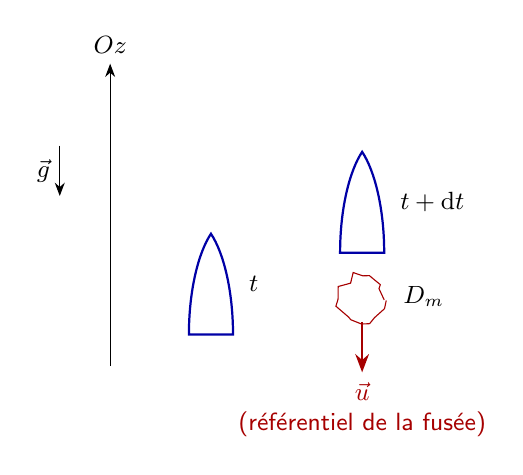
\begin{tikzpicture}[scale=.8]
\draw[->](0,-.5)--(0,4.3)node[above]{$Oz$};\draw[->](-.8,3)--(-.8,2.2)node[midway,left]{$\vec g$};
\foreach\x/\y/\lab in{1.6/0/t,4/1.3/{t+\dd t}}{\draw[blue!65!black,thick](\x,\y)--++(-.35,0)..controls(\x-.35,\y+.7)and(\x-.2,\y+1.3)..(\x,\y+1.6)..controls(\x+.2,\y+1.3)and(\x+.35,\y+.7)..(\x+.35,\y)--cycle;\node[right]at(\x+.45,\y+.8){$\lab$};}
\draw[red!65!black,decorate,decoration={random steps,segment length=3pt,amplitude=2pt}](4,.55)circle(.35);\node[right]at(4.5,.6){$D_m$};\draw[force](4,.2)--(4,-.6)node[below,align=center]{$\vec u$\\(référentiel de la fusée)};
\end{tikzpicture}\end{center}
\par\textbf{Hypothèses :}
\begin{itemize}
\item Le référentiel est le référentiel terrestre, supposé galiléen.
\end{itemize}
\etape{1) Système fermé et forces extérieures}
Le système fermé $\Sigma$ comprend :
\begin{itemize}\item à $t$, la fusée et tout ce qu'elle contient ;\item à $t+\dd t$, la fusée et tout ce qu'elle contient, ainsi que les gaz éjectés pendant $\dd t$, de masse $D_m\dd t$.\end{itemize}
$m(t)$ est la masse de la fusée et de tout ce qu'elle contient ; $\vec v(t)$ est sa vitesse. Ces grandeurs sont associées à un système ouvert.
\par\par\par\medskip\noindent\begin{minipage}{\linewidth}
\textbf{Forces extérieures :}
\begin{itemize}
\item Le poids.
\item Les forces de pression $\vec F_{\mathrm{pression}}\simeq\vec0$ (la poussée d'Archimède $\vec\Pi_A\simeq\vec0$ dans l'air).
\item Les frottements fluides, négligés.
\end{itemize}
\end{minipage}\par
\etape{2) Bilan de quantité de mouvement}
\[\vec p_\Sigma(t)=m(t)\vec v(t),\]
\[\vec p_\Sigma(t+\dd t)=m(t+\dd t)\vec v(t+\dd t)+D_m\dd t\bigl[\vec u+\vec v(t+\dd t)\bigr].\]
\begin{align*}
\dd\vec p_\Sigma&=m(t+\dd t)\vec v(t+\dd t)-m(t)\vec v(t)+D_m\dd t\bigl(\vec u+\vec v(t+\dd t)\bigr)\\
&=\frac{\dd}{\dd t}\bigl(m(t)\vec v(t)\bigr)\dd t+D_m\dd t\bigl(\vec u+\vec v(t)\bigr)\\
&=\underbrace{\frac{\dd m}{\dd t}}_{-D_m}\vec v(t)\dd t+m(t)\frac{\dd\vec v}{\dd t}\dd t+D_m\dd t\bigl(\vec u+\vec v(t)\bigr).
\end{align*}
Calcul limité à l'ordre 1 en $\dd t$ : $\vec v(t+\dd t)=\vec v(t)+\dd t\,\dd\vec v/\dd t+\cdots$.
\begin{cadre}\[\dd\vec p_\Sigma=m(t)\frac{\dd\vec v}{\dd t}\dd t+D_m\dd t\,\vec u.\]\end{cadre}
\etape{3) Théorème de la quantité de mouvement}
\[\dd\vec p_\Sigma=m_\Sigma\vec g\,\dd t=m(t)\vec g\,\dd t,\]
\[m(t)\frac{\dd\vec v}{\dd t}\dd t+D_m\vec u\,\dd t=m(t)\vec g\,\dd t.\]
\begin{cadre}\[m(t)\frac{\dd\vec v}{\dd t}=m(t)\vec g\underbrace{-D_m\vec u}_{\text{force de poussée}}.\]\end{cadre}
La condition de décollage est $D_m u>m(0)g$.
\par\medskip\noindent\textbf{Application numérique :} $u\sim\mathrm{km\,s^{-1}}$ et $D_m u\sim3\times10^7\,\mathrm N$.
\end{exemple}
\subsection{Coude de canalisation}
% Sources 9-13
\begin{exemple}[breakable]
\begin{center}\coude{0}\end{center}
\par\textbf{Hypothèses :}
\begin{itemize}
\item L'écoulement est parfait, incompressible et stationnaire.
\item La pesanteur est négligée.
\end{itemize}
L'incompressibilité, la section constante et le caractère parfait de l'écoulement donnent $Sv=\cste$ ($v$ constante sur une section), donc
\begin{cadre}\[v_1=v_2=v.\]\end{cadre}
Le théorème de Bernoulli entre $A$ et $B$, pour un écoulement incompressible, stationnaire et homogène, donne
\[P_1+\frac12\mu v^2=P_2+\frac12\mu v^2.\]
\begin{cadre}\[P_1=P_2=P.\]\end{cadre}
\par\noindent\begin{minipage}{\linewidth}
\etape{1) Système fermé et forces extérieures}
\begin{center}\coude{1}\end{center}
\end{minipage}\par
$\Sigma$ est un système fermé constitué de fluide :
\begin{itemize}
\item À $t$, il comprend le fluide dans $\sys$ et le fluide qui entre entre $t$ et $t+\dd t$, de masse $D_m\dd t$.
\item À $t+\dd t$, il comprend le fluide dans $\sys$ et le fluide qui sort pendant cet intervalle, de masse $D_m\dd t$.
\end{itemize}
\par\par\par\medskip\noindent\begin{minipage}{\linewidth}
\textbf{Forces extérieures :}
\begin{itemize}
\item Le poids, négligé.
\item Les forces de pression en amont et en aval ($P_1=P_2=P$).
\item La force du tuyau sur le fluide : $\vec F_{\mathrm{tuyau}\to\mathrm{eau}}=-\vec F_{\mathrm{eau}\to\mathrm{tuyau}}=-\vec F$.
\end{itemize}
\end{minipage}\par
\etape{2) Bilan de quantité de mouvement}
\[\vec p_\Sigma(t)=\vec p_{\sys}(t)+D_m\dd t\,v\ux,\qquad
\vec p_\Sigma(t+\dd t)=\vec p_{\sys}(t+\dd t)+D_m\dd t\,v\uy.\]
\begin{cadre}\[\dd\vec p_\Sigma=\underbrace{\dd\vec p_{\sys}}_{\vec0\text{ : écoulement stationnaire}}+D_m\dd t\,v(\uy-\ux).\]\end{cadre}
\etape{3) Théorème de la quantité de mouvement}
\[\dd\vec p_\Sigma=\vec F_{\mathrm{ext}}\dd t,\qquad D_m\dd t\,v(\uy-\ux)=-\vec F\dd t+(PS\ux-PS\uy)\dd t.\]
\[\vec F=PS(\ux-\uy)-D_m v(\uy-\ux)=(PS+D_m v)(\ux-\uy).\]
\begin{cadre}\[\vec F=S(P+\mu v^2)(\ux-\uy).\]\end{cadre}
\textbf{Remarques :} le sens et la direction sont cohérents avec les prévisions. La force augmente lorsque $P$, $v$ ou $S$ augmente.
\par\medskip\noindent\textbf{Application numérique :} pour un tuyau de diamètre $D=20\,\mathrm{cm}$, avec $P=6\,\mathrm{bar}$ et $D_V=0{,}2\,\mathrm{m^3\,s^{-1}}$, on obtient $F=2\times10^4\,\mathrm N$ : la force est très importante. \\
\titr{Effet Coanda}
\begin{center}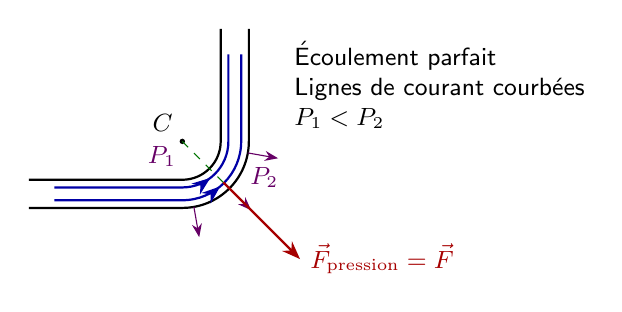
\begin{tikzpicture}[scale=.65]
\draw[thick](0,0)--(3,0)arc(-90:0:1.3)--(4.3,3.5);\draw[thick](0,.55)--(3,.55)arc(-90:0:.75)--(3.75,3.5);
\foreach\d in{.15,.4}{\draw[courant](.5,\d)--(3,\d)arc(-90:0:{1.3-\d})--({4.3-\d},3);}
\fill(3,1.3)circle(1.5pt)node[above left]{$C$};\draw[dashed,green!45!black](3,1.3)--(4.4,-.1);
\foreach\a in{-80,-45,-10}{\draw[pression,->]({3+1.3*cos(\a)},{1.3+1.3*sin(\a)})--({3+1.9*cos(\a)},{1.3+1.9*sin(\a)});}
\node[pression]at(2.6,1){$P_1$};\node[pression]at(4.6,.6){$P_2$};\draw[force](3.8,.5)--(5.3,-1)node[right]{$\vec F_{\mathrm{pression}}=\vec F$};\node[right,align=left]at(5,2.4){Écoulement parfait\\Lignes de courant courbées\\$P_1<P_2$};
\end{tikzpicture}\end{center}
Réciproquement, on peut interpréter l'effet Coanda par un bilan de quantité de mouvement.
\begin{center}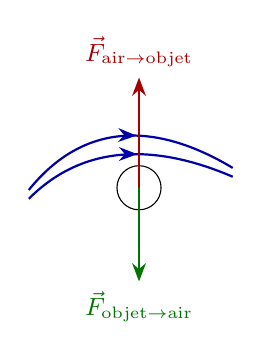
\begin{tikzpicture}[scale=.7]
\draw(0,0)circle(.4);\foreach\h in{.8,1.2}{\draw[courant](-2,{-.2+.4*(\h-.8)})..controls(-1,\h)and(.3,\h)..(1.7,{.2+.4*(\h-.8)});}\draw[force](0,0)--(0,2)node[above]{$\vec F_{\mathrm{air}\to\mathrm{objet}}$};\draw[green!45!black,->,thick](0,0)--(0,-1.7)node[below]{$\vec F_{\mathrm{objet}\to\mathrm{air}}$};
\end{tikzpicture}\end{center}
\end{exemple}
\Needspace{75mm}
\subsection{Jet cylindrique sur une plaque}
% Sources 13-20
\begin{exemple}[breakable]
\begin{center}\jet{0}\end{center}
\par\textbf{Hypothèses :}
\begin{itemize}\item La pesanteur est négligée.
\item Le jet est libre : $P=P_0$ partout.
\item L'écoulement est parfait, incompressible, stationnaire et homogène. Le théorème de Bernoulli entre $A$ et $B$ donne
\[\frac12\mu v_0^2+P_0=\frac12\mu v_B^2+P_0,\qquad\boxed{v_B=v_0}.\]
\item Le débit volumique se conserve à travers toute section du tube de courant global :
\[v_0S=v_0\,2\pi Re\quad\Longrightarrow\quad S=2\pi Re.\]
\item L'écoulement est stationnaire : $D_m=\mu Sv_0$.\end{itemize}
\par\noindent\begin{minipage}{\linewidth}
\etape{1) Système fermé et forces extérieures}
\begin{center}\begin{minipage}{.48\linewidth}\centering\jet{1}\end{minipage}\hfill\begin{minipage}{.48\linewidth}\centering\jet{2}\end{minipage}\end{center}
\end{minipage}\par
$\sys$ est un système ouvert fixe et indéformable.
\par Le système fermé $\Sigma$, constitué de fluide, comprend :
\begin{itemize}\item à $t$, le fluide contenu dans $\sys(t)$ et le fluide qui entre dans $\sys$ entre $t$ et $t+\dd t$ ;
\item à $t+\dd t$, le fluide contenu dans $\sys(t)$ et le fluide qui sort de $\sys$ entre $t$ et $t+\dd t$.\end{itemize}
\par\par\par\medskip\noindent\begin{minipage}{\linewidth}
\textbf{Forces extérieures :}
\begin{itemize}
\item Le poids, négligé.
\item Les forces de pression eau/eau en amont et en aval à $P_0$.
\item Les forces de pression air/eau latérales à $P_0$.
\item La force $\vec F_{\mathrm{disque}\to\mathrm{eau}}$.
\end{itemize}
\end{minipage}\par
\etape{2) Bilan de quantité de mouvement}
\[\vec p_\Sigma(t)=\vec p_{\sys}(t)+D_m\dd t\,v_0\ux,\qquad\vec p_\Sigma(t+\dd t)=\vec p_{\sys}(t+\dd t)+\vec0.\]
La résultante de la quantité de mouvement de l'eau sortante est nulle :
\begin{center}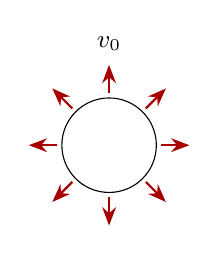
\begin{tikzpicture}[scale=.6]\draw(0,0)circle(1);\foreach\a in{0,45,...,315}{\draw[force](\a:1.1)--(\a:1.7);}\node[above]at(0,1.8){$v_0$};\end{tikzpicture}\end{center}
\[\dd\vec p_\Sigma=\underbrace{\dd\vec p_{\sys}}_{\vec0\text{ : stationnaire}}-\underbrace{D_m}_{\mu Sv_0}\dd t\,v_0\ux.\]
\begin{cadre}\[\dd\vec p_\Sigma=-\mu Sv_0^2\ux\,\dd t.\]\end{cadre}
\etape{3) Théorème de la quantité de mouvement}
Dans le référentiel terrestre galiléen,
\[\dd\vec p_\Sigma=-\mu Sv_0^2\ux\,\dd t=\bigl(\vec F_{\mathrm{plaque}\to\mathrm{eau}}+\vec F_{\mathrm{tot\,pression}}\bigr)\dd t.\]
\titr{Calcul de la résultante des forces de pression}
\begin{center}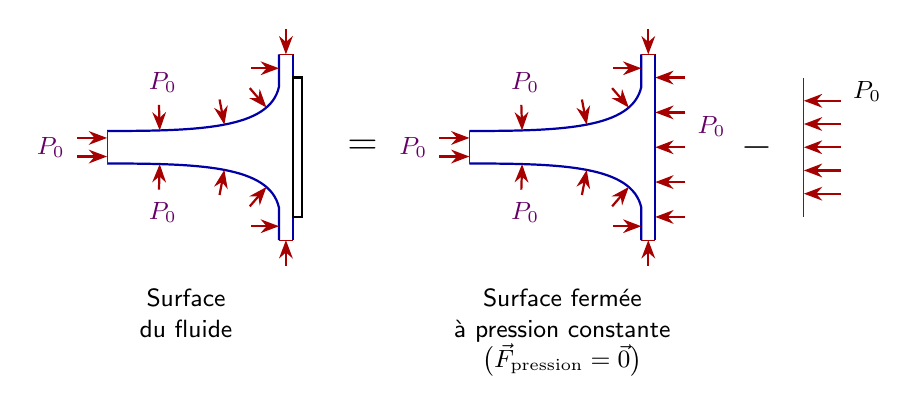
\begin{tikzpicture}[scale=.59]
\foreach \shift/\closed in {0/0,7.8/1}{
\begin{scope}[xshift=\shift cm]
\jetbase
\draw[red!65!black](0,-.35)--(0,.35)(3.7,2)--(4,2)(3.7,-2)--(4,-2);
\foreach \y in {-.2,.2}{\draw[force](-.65,\y)--(0,\y);}
\foreach \t in {.2,.5,.8}{
\pgfmathsetmacro{\px}{6*(1-\t)^2*\t+10.5*(1-\t)*\t^2+3.7*\t^3}
\pgfmathsetmacro{\py}{.35*(1-\t)^3+1.05*(1-\t)^2*\t+1.2*(1-\t)*\t^2+1.3*\t^3}
\pgfmathsetmacro{\dx}{6*(1-\t)^2+9*(1-\t)*\t+.6*\t^2}
\pgfmathsetmacro{\dy}{.3*(1-\t)*\t+2.7*\t^2}
\pgfmathsetmacro{\nn}{sqrt(\dx*\dx+\dy*\dy)}
\draw[force]({\px-.55*\dy/\nn},{\py+.55*\dx/\nn})--(\px,\py);
\draw[force]({\px-.55*\dy/\nn},{-\py-.55*\dx/\nn})--(\px,-\py);
}
\foreach \y in {-1.7,1.7}{\draw[force](3.1,\y)--(3.7,\y);}
\draw[force](3.85,2.55)--(3.85,2);\draw[force](3.85,-2.55)--(3.85,-2);
\node[pression]at(1.2,1.4){$P_0$};\node[pression]at(1.2,-1.4){$P_0$};\node[pression,left]at(-.7,0){$P_0$};
\ifnum\closed=0
\draw[thick](4,-1.5)rectangle(4.2,1.5);
\node[below,align=center]at(1.7,-2.85){Surface\\du fluide};
\else
\foreach\y in{-1.5,-.75,0,.75,1.5}{\draw[force](4.65,\y)--(4,\y);}
\node[pression,right]at(4.7,.45){$P_0$};
\node[below,align=center]at(2,-2.85){Surface fermée\\à pression constante\\$\bigl(\vec F_{\mathrm{pression}}=\vec0\bigr)$};
\fi
\end{scope}}
\node[font=\Large]at(5.5,0){$=$};
\node[font=\Large]at(14,0){$-$};
\draw[red!65!black](15,-1.5)--(15,1.5);
\foreach\y in{-1,-.5,0,.5,1}{\draw[force](15.8,\y)--(15,\y);}
\node[right]at(15.85,1.2){$P_0$};
\end{tikzpicture}\end{center}
\[\vec F_{\mathrm{tot\,pression}}=\vec0-\bigl(-P_0\pi R^2\ux\bigr)=P_0\pi R^2\ux.\]
D'où
\[-\mu Sv_0^2\ux\,\dd t=\bigl(P_0\pi R^2\ux-\vec F_{\mathrm{eau}\to\mathrm{plaque}}\bigr)\dd t.\]
\begin{cadre}\[\vec F_{\mathrm{eau}\to\mathrm{plaque}}=(P_0\pi R^2+\mu Sv_0^2)\ux.\]\end{cadre}
Cette force est dirigée selon $\ux$. Elle augmente avec $v_0$, $S$ et $\mu$. \\
\titr{Détermination de $\vec F_{\mathrm{op}}$}
Le système $\Sigma'$ est la plaque à l'équilibre.
\begin{center}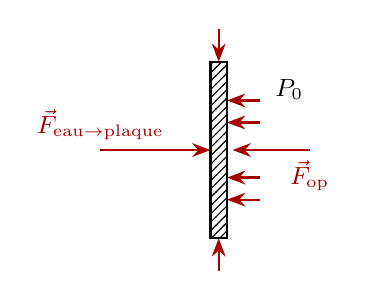
\begin{tikzpicture}[scale=.7]
\fill[pattern=north east lines](0,-1.6)rectangle(.3,1.6);\draw[thick](0,-1.6)rectangle(.3,1.6);\draw[force](-2,0)--(0,0)node[pos=0,above]{$\vec F_{\mathrm{eau}\to\mathrm{plaque}}$};\draw[force](1.8,0)--(.4,0)node[pos=0,below]{$\vec F_{\mathrm{op}}$};\foreach\y in{-.9,-.5,.5,.9}{\draw[force](.9,\y)--(.3,\y);}\draw[force](.15,2.2)--(.15,1.6);\draw[force](.15,-2.2)--(.15,-1.6);\node[right]at(1,1.1){$P_0$};
\end{tikzpicture}\end{center}
Le théorème de la quantité de mouvement donne
\[\vec0=\vec F_{\mathrm{eau}\to\mathrm{plaque}}+\vec F_{\mathrm{op}}+\underbrace{\vec F_{\mathrm{pression}}}_{\vec0-\pi R^2P_0\ux},\]
\[\vec F_{\mathrm{op}}=\pi R^2P_0\ux-(P_0\pi R^2+\mu Sv_0^2)\ux.\]
\begin{cadre}\[\vec F_{\mathrm{op}}=-\mu Sv_0^2\ux.\]\end{cadre}
$\vec F_{\mathrm{op}}$ est dirigée selon $-\ux$ et sa norme augmente avec $\mu$, $S$ et $v_0$.
\titr{Remarque : choix du système}
On a appliqué le théorème de la quantité de mouvement à $\Sigma$, puis à $\Sigma'$. Il aurait été préférable de choisir $\Sigma''=\Sigma\cup\Sigma'$, c'est-à-dire le fluide et la plaque.
\par\noindent\begin{minipage}{\linewidth}
\etape{1) Système et forces extérieures}
\begin{center}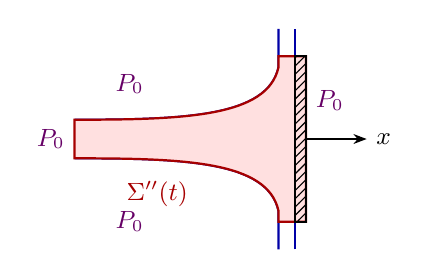
\begin{tikzpicture}[scale=.7]\jetbase
\fill[red!12](0,-.35)..controls(2,-.35)and(3.5,-.4)..(3.7,-1.3)--(3.7,-1.5)--(4.2,-1.5)--(4.2,1.5)--(3.7,1.5)--(3.7,1.3)..controls(3.5,.4)and(2,.35)..(0,.35)--cycle;\draw[red!65!black,thick](0,-.35)..controls(2,-.35)and(3.5,-.4)..(3.7,-1.3)--(3.7,-1.5)--(4.2,-1.5)--(4.2,1.5)--(3.7,1.5)--(3.7,1.3)..controls(3.5,.4)and(2,.35)..(0,.35)--cycle;\fill[pattern=north east lines](4,-1.5)rectangle(4.2,1.5);\draw[thick](4,-1.5)rectangle(4.2,1.5);\node[red!65!black]at(1.5,-1){$\Sigma''(t)$};\node[pression]at(1,1){$P_0$};\node[pression,left]at(0,0){$P_0$};\node[pression]at(1,-1.5){$P_0$};\node[pression,right]at(4.2,.7){$P_0$};\draw[->](4.2,0)--(5.3,0)node[right]{$x$};\end{tikzpicture}\end{center}
\end{minipage}\par
\par\par\par\medskip\noindent\begin{minipage}{\linewidth}
\textbf{Forces extérieures :}
\begin{itemize}
\item La force $\vec F_{\mathrm{op}}$.
\item Les forces de pression, dont la résultante est nulle ($P_0$ partout).
\item Le poids, négligé.
\end{itemize}
\end{minipage}\par
\etape{2) Variation de quantité de mouvement}
\[\dd\vec p_{\Sigma''}=\underbrace{\dd\vec p_{\Sigma'}}_{\vec0}+\dd\vec p_\Sigma=-\mu Sv_0^2\ux\,\dd t.\]
\etape{3) Théorème de la quantité de mouvement}
\[-\mu Sv_0^2\ux\,\dd t=\vec F_{\mathrm{op}}\dd t.\]
\begin{cadre}\[\vec F_{\mathrm{op}}=-\mu Sv_0^2\ux.\]\end{cadre}
\begin{cadre}
En fonction de la question posée, il peut être intéressant d'inclure l'obstacle dans le système.
\begin{itemize}\item On applique une seule fois le théorème de la quantité de mouvement au lieu de deux.
\item Le calcul de la résultante des forces de pression est plus facile.
\item On évite de calculer $\vec F_{\mathrm{eau}\to\mathrm{plaque}}$, qui est une force intérieure pour $\Sigma''$.\end{itemize}
\end{cadre}
\end{exemple}
\section{Bilan d'énergie}
% Sources 20-22
\titr{Rappel de première année}
Pour un système fermé, on utilise en mécanique le théorème de l'énergie mécanique, et en thermodynamique le premier principe.
\[\frac{\dd E_m}{\dd t}=\Piext+\Piint,\qquad \dd E_{m,\mathrm{macroscopique}}+\dd U=\delta W_{\mathrm{ext}}+\delta Q.\]
$Q$ représente les échanges microscopiques. Pour les forces intérieures,
\[\dd U=\dd E_{c,\mathrm{microscopique}}+\dd E_{p,\text{intérieur}},\]
sous l'hypothèse que toutes les forces intérieures sont conservatives.
\titr{En mécanique des fluides}
S'il y a un échange de chaleur ou si l'écoulement est compressible, on peut appliquer le premier principe industriel.
\newpage
\titr{Méthodologie}
\begin{enumerate}\item Définir le système $\Sigma$ \textbf{fermé}, effectuer le bilan des forces extérieures et intérieures, puis leur caractérisation énergétique.
\item Faire le bilan d'énergie mécanique ou cinétique.
\item Appliquer le théorème de l'énergie cinétique ou le théorème de l'énergie mécanique à $\Sigma$.\end{enumerate}
\subsection{Interprétation énergétique du théorème de Bernoulli}
% Sources 22-28
\titr{Hypothèses}
\begin{itemize}
\item L'écoulement est parfait : il n'y a pas de viscosité ni d'échange de chaleur.
\item Il est stationnaire : les lignes de courant coïncident avec les trajectoires.
\end{itemize}
On considère un tube de courant élémentaire, avec deux sections élémentaires $S_A$ et $S_B$.
\begin{center}\streamtube{0}\end{center}
\par\noindent\begin{minipage}{\linewidth}
\etape{1) Système et bilan des forces}
\begin{center}\begin{minipage}{.48\linewidth}\centering\streamtube{1}\end{minipage}\hfill\begin{minipage}{.48\linewidth}\centering\streamtube{2}\end{minipage}\end{center}
\end{minipage}\par
$\sys$ est ouvert, fixe et indéformable.
\par $\Sigma$ est une portion fermée de fluide :
\begin{itemize}\item à $t$, elle comprend le fluide contenu dans $\sys$ à $t$ et le fluide entrant dans $\sys$ entre $t$ et $t+\dd t$ ;
\item à $t+\dd t$, elle comprend le fluide contenu dans $\sys$ à $t+\dd t$ et le fluide sortant de $\sys$ entre $t$ et $t+\dd t$.\end{itemize}
\par\par\medskip\noindent\begin{minipage}{\linewidth}
\textbf{Forces extérieures :}
\begin{itemize}\item Les forces à distance $\vec f_v$ sont supposées conservatives. On note $E_{pV}$ l'énergie potentielle volumique et $E_{pm}$ l'énergie potentielle massique : $E_{pV}=\mu E_{pm}$.
\item Les forces de pression en amont et en aval, $P_A$ et $P_B$, fournissent les travaux d'admission et de refoulement.
\item Les forces de pression latérales ne travaillent pas : $\vec F\perp\vec v$.\end{itemize}
\end{minipage}\par
\par\par\par\medskip\noindent\begin{minipage}{\linewidth}
\textbf{Forces intérieures :}
\begin{itemize}
\item Les forces de pression intérieures.
\item On s'interroge sur un éventuel autre travail.
\end{itemize}
\end{minipage}\par
\etape{2) Bilan d'énergie}
\[E_{c\Sigma}(t)=E_{c\sys}(t)+D_m\dd t\,\frac12v_A^2,\qquad E_{c\Sigma}(t+\dd t)=E_{c\sys}(t+\dd t)+D_m\dd t\,\frac12v_B^2.\]
\textbf{Remarque :} l'écoulement est stationnaire, donc $D_m=\mu_AS_Av_A=\mu_BS_Bv_B$ est le même à travers toute section du tube de courant considéré.
\begin{cadre}\[\dd E_{c\Sigma}=\underbrace{\dd E_{c\sys}}_{0}+D_m\dd t\left(\frac12v_B^2-\frac12v_A^2\right).\]\end{cadre}
\[E_{p\Sigma}(t)=E_{p\sys}(t)+D_m\dd t\,E_{pm}(A),\]
\[E_{p\Sigma}(t+\dd t)=E_{p\sys}(t+\dd t)+D_m\dd t\,E_{pm}(B),\]
\[\dd E_{p\Sigma}=\underbrace{\dd E_{p\sys}}_{0}+D_m\dd t\bigl(E_{pm}(B)-E_{pm}(A)\bigr).\]
\begin{cadre}\[\dd E_{p\Sigma}=D_m\dd t\bigl(E_{pm}(B)-E_{pm}(A)\bigr).\]\end{cadre}
\etape{3) Théorème de l'énergie mécanique entre $t$ et $t+\dd t$}
\[\frac{\dd E_m}{\dd t}=\Piint+\Piext,\]
\[\dd E_{c\Sigma}+\dd E_{p\Sigma}=\Piint\dd t+\underbrace{P_AS_Av_A\dd t}_{\text{travail d'admission}}-\underbrace{P_BS_Bv_B\dd t}_{\text{travail de refoulement}}.\]
\[
D_m\dd t\left[E_{pm}(B)+\frac12v_B^2-\left(E_{pm}(A)+\frac12v_A^2\right)\right]=\Piint\dd t+\left(\frac{P_AD_m}{\mu_A}-\frac{P_BD_m}{\mu_B}\right)\dd t.
\]
\begin{cadre}\[D_m\left[\left(E_{pm}(B)+\frac12v_B^2+\frac{P_B}{\mu_B}\right)-\left(E_{pm}(A)+\frac12v_A^2+\frac{P_A}{\mu_A}\right)\right]=\Piint.\]\end{cadre}
Dans le cours précédent, pour un écoulement parfait, stationnaire, incompressible et homogène,
\[P+\frac12\mu v^2+E_{pV}=\cste.\]
Si l'on ajoute l'hypothèse d'incompressibilité, $\mu$ est constante sur une trajectoire. Or les trajectoires coïncident avec les lignes de courant : $\mu_A=\mu_B=\mu$. Ainsi,
\[D_m\left[\left(\frac12\mu v_B^2+P_B+E_{pV}(B)\right)-\left(\frac12\mu v_A^2+P_A+E_{pV}(A)\right)\right]=\mu\Piint.\]
Avec le théorème de Bernoulli, on déduit $\Piint=0$ pour un écoulement incompressible.
\begin{cadre}\begin{enumerate}\item Le théorème de Bernoulli traduit la conservation de l'énergie.
\item Dans un écoulement parfait, stationnaire et incompressible, la puissance des forces intérieures de pression est nulle.\end{enumerate}\end{cadre}
\textbf{Remarque :} on généralisera le résultat à tout écoulement incompressible.
\begin{cadre}[etoiles={\etoiles{2}}]Dans un écoulement incompressible, la puissance des forces intérieures de pression est nulle.\end{cadre}
Si l'écoulement est compressible, il faut connaître $\Piint$ : il faut utiliser le premier principe thermodynamique,
\[\dd E_{m,\mathrm{macroscopique}}+\dd U=\underbrace{\delta W_{\mathrm{ext}}}_{\text{pression en amont et en aval}}+\underbrace{\delta Q}_{\text{supposé nul}}.\]
Dans l'égalité précédente, les variations d'énergie mécanique macroscopique correspondent aux termes $E_{pm}+v^2/2$, le travail de pression aux termes $P/\mu$, et la variation d'énergie interne au terme $\Piint$.
\begin{exemple}[breakable]
\textbf{Exercice 6, TD F4}
% Sources 28-33
\begin{center}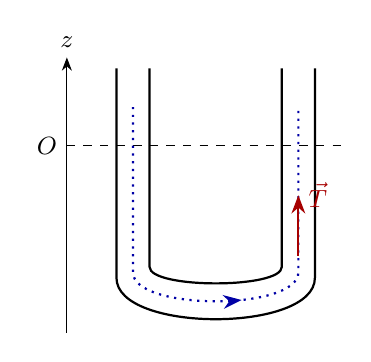
\begin{tikzpicture}[scale=.7]
\draw[->](-2.7,-1.8)--(-2.7,3.2)node[above]{$z$};\node[left]at(-2.7,1.6){$O$};\draw[dashed](-2.7,1.6)--(2.3,1.6);
\draw[thick](-1.8,3)--(-1.8,-.8)..controls(-1.8,-1.8)and(1.8,-1.8)..(1.8,-.8)--(1.8,3);\draw[thick](-1.2,3)--(-1.2,-.6)..controls(-1.2,-1)and(1.2,-1)..(1.2,-.6)--(1.2,3);
\draw[courant,dotted](-1.5,2.3)--(-1.5,-.7)..controls(-1.5,-1.4)and(1.5,-1.4)..(1.5,-.7)--(1.5,2.3);\draw[force](1.5,-.4)--(1.5,.7)node[right]{$\vec T$};
\end{tikzpicture}\end{center}
\par\textbf{Hypothèses :}
\begin{itemize}
\item Le fluide est incompressible : $\rho=\cste$.
\item Le volume $V=SL$ et la section $S$ sont constants.
\item L'écoulement est unidimensionnel, $\vec v(M,t)=v(M,t)\vec T$, et parfait.
\end{itemize}
L'incompressibilité impose que $D_V$ soit constant à travers toute section du tube : pour tout $M$, $Sv(M,t)=\cste$. La vitesse scalaire est donc indépendante de $M$.
\begin{cadre}\[\vec v(M,t)=v(t)\vec T.\]\end{cadre}
\titr{Méthode énergétique}
\etape{1) Système et bilan des forces}
Le système est tout le liquide.
\begin{center}\utube{1}\end{center}
Le fluide est incompressible : si le niveau à droite est $z$, le niveau à gauche est $-z$. Il y a un degré de liberté.
Dans le référentiel terrestre galiléen, les forces extérieures sont :
\begin{itemize}\item le poids, conservatif ;
\item les forces de pression air/eau à $P_0$, dont les travaux sont $P_0S(-\dd z)$ à droite et $P_0S\dd z$ à gauche ; ainsi $W_{\mathrm{pression}}=0$ ;
\item les forces de contact normales des parois, dont le travail est nul car $\vec F\perp\vec v$.\end{itemize}
\par\par\par\medskip\noindent\begin{minipage}{\linewidth}
\textbf{Forces intérieures :}
\begin{itemize}
\item Les forces de pression : leur travail $W_{\mathrm{int}}$ est nul car l'écoulement est incompressible.
\end{itemize}
\end{minipage}\par
Le système est conservatif, à un degré de liberté : $E_m=\cste$.
\par\noindent\begin{minipage}{\linewidth}
\Needspace{35mm}
\etape{2) Calcul des énergies}
\titr{Énergie cinétique}
$\vec v(M,t)=v(t)\vec T$ ; la valeur de $v(t)$ est la même en tout point.
\[E_c=\iiint_V\frac12\mu v^2(t)\,\dd^3\tau=\frac12\mu v^2(t)\iiint_V\dd^3\tau.\]
\begin{cadre}\[E_c=\frac12\mu SLv^2(t).\]\end{cadre}
\end{minipage}\par
\par\noindent\begin{minipage}{\linewidth}
    
\titr{Énergie potentielle}
Il s'agit ici de l'énergie potentielle du poids.
\begin{center}\begin{minipage}{.48\linewidth}\centering\utube{0}\par Valeur de référence : $E_p=0$.\end{minipage}\hfill\begin{minipage}{.48\linewidth}\centering\utube{1}\end{minipage}\end{center}
\end{minipage}\par
\[E_p=0+\mu Szg\left(\frac z2\right)-\mu Szg\left(-\frac z2\right).\]
\begin{cadre}\[E_p=\mu Sz^2g.\]\end{cadre}
\etape{3) Théorème de l'énergie mécanique}
\[E_m=\cste=\frac12\mu SLv^2(t)+\mu Sgz^2,\qquad v(t)=\dot z(t).\]
\begin{cadre}\[\frac12\mu SL\dot z^2+\mu Sgz^2=E_m.\]\end{cadre}
On dérive par rapport au temps :
\[\frac{\dd E_m}{\dd t}=\frac12\mu SL(2\dot z\ddot z)+\mu Sg(2z\dot z)=0.\]
\begin{cadre}\[\ddot z+\frac{2g}{L}z=0.\]\end{cadre}
La solution est de la forme $z(t)=A\cos(\omega t+\varphi)$.
\begin{cadre}Les oscillations sont sinusoïdales, de pulsation $\displaystyle\omega=\sqrt{\frac{2g}{L}}$.\end{cadre}
En réalité, il faut tenir compte de la viscosité.
\par\textbf{Remarque :} une deuxième méthode utilise l'équation d'Euler ; cf. TD.
\end{exemple}
\Needspace{65mm}
\begin{exemple}[breakable]
\textbf{TD 3, exercice 7}
% Sources 33-36
\begin{center}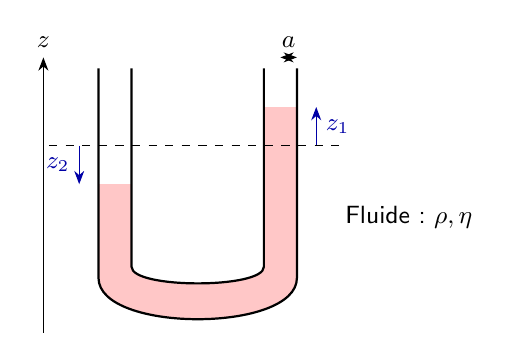
\begin{tikzpicture}[scale=.7]
\draw[->](-2.8,-1.8)--(-2.8,3.2)node[above]{$z$};
\fill[red!22](-1.8,.9)--(-1.8,-.8)..controls(-1.8,-1.8)and(1.8,-1.8)..(1.8,-.8)--(1.8,2.3)--(1.2,2.3)--(1.2,-.6)..controls(1.2,-1)and(-1.2,-1)..(-1.2,-.6)--(-1.2,.9)--cycle;
\draw[thick](-1.8,3)--(-1.8,-.8)..controls(-1.8,-1.8)and(1.8,-1.8)..(1.8,-.8)--(1.8,3);\draw[thick](-1.2,3)--(-1.2,-.6)..controls(-1.2,-1)and(1.2,-1)..(1.2,-.6)--(1.2,3);\draw[->,blue!65!black](2.15,1.6)--(2.15,2.3)node[midway,right]{$z_1$};\draw[->,blue!65!black](-2.15,1.6)--(-2.15,.9)node[midway,left]{$z_2$};\draw[<->](1.5,3.2)--(1.8,3.2)node[midway,above]{$a$};\node[right]at(2.5,.3){Fluide : $\rho,\eta$};\draw[dashed](-2.7,1.6)--(2.6,1.6);
\end{tikzpicture}\end{center}
\[\vec v(M,t)=v(r,t)\vec T=v_0(t)\left(1-\frac{r^2}{a^2}\right)\vec T.\]
\par\textbf{Hypothèses :}
\begin{itemize}
\item Il s'agit d'un écoulement de Poiseuille cylindrique.
\item Le fluide est incompressible.
\end{itemize}
On a toujours $D_V=\pi a^2\dot z_1=\cste$ et
\[\pi a^2\dot z_1=-\pi a^2\dot z_2\quad\Longrightarrow\quad z_1=-z_2.\]
\[D_V=\int_0^a2\pi r\,\dd r\,v_0(t)\left(1-\frac{r^2}{a^2}\right)=\pi a^2v_{\mathrm{moy}}.\]
\begin{cadre}\[v_{\mathrm{moy}}=\dot z_1=\frac{v_0(t)}2.\]\end{cadre}
Le problème a un degré de liberté.
\etape{1) Système et bilan des forces}
Le système est tout le liquide.
\par\par\medskip\noindent\begin{minipage}{\linewidth}
\textbf{Forces extérieures :}
\begin{itemize}\item Le poids est conservatif.
\item Le travail des forces de pression air/eau est nul.
\item Le travail des forces de contact normales tube/liquide est nul.
\item Le travail des forces de viscosité tube/liquide est nul : le liquide adhère au tube, donc $\vec v=\vec0$ aux parois.\end{itemize}
\end{minipage}\par
\par\par\medskip\noindent\begin{minipage}{\linewidth}
\textbf{Forces intérieures :}
\begin{itemize}\item Le travail des forces de pression est nul car l'écoulement est incompressible.
\item Le travail des forces de viscosité est non nul. On admet
\[\Piint=-8\pi\eta\ell\dot z_1^2.\]\end{itemize}
\end{minipage}\par
\etape{2) Calcul des énergies}
Par le même calcul que précédemment, $E_p=\rho Sgz_1^2$.
\begin{align*}
E_c&=\iiint_V\frac12\rho v^2(r,t)\,\dd^3\tau\\
&=\ell\rho\int_0^a\frac12v^2(r,t)\,2\pi r\,\dd r\\
&=\frac12\ell(2\pi\rho)\int_0^av^2(r,t)r\,\dd r\\
&=\ell\rho\pi\int_0^av_0^2(t)\left(1-\frac{r^2}{a^2}\right)^2r\,\dd r.
\end{align*}
\begin{cadre}\[E_c=\ell\rho\pi v_0^2(t)\frac{a^2}{6},\qquad v_0=2\dot z_1.\]\end{cadre}
\etape{3) Théorème de l'énergie mécanique}
\[\frac{\dd E_m}{\dd t}=\Piint=-8\pi\eta\ell\dot z_1^2,\]
\[\rho\ell\pi a^2\frac43\dot z_1\ddot z_1+2\rho g\pi a^2z_1\dot z_1=-8\pi\eta\ell\dot z_1^2.\]
\begin{cadre}\[\ddot z_1+\frac{6\eta}{\rho a^2}\dot z_1+\frac{3g}{2\ell}z_1=0.\]\end{cadre}
\[\omega_0^2=\frac{3g}{2\ell},\qquad\frac{\omega_0}{Q}=\frac{6\eta}{\rho a^2}.\]
Pour l'eau, $Q=28$ : le régime est pseudo-périodique. Pour l'huile, $Q<1/2$ : le régime est apériodique. \\

\textbf{Remarque :} la formule $\Piint=-8\pi\eta\ell\dot z_1^2$ est celle d'un tube droit. En réalité, les amortissements dus à la viscosité sont plus importants dans le tube courbé.
\end{exemple}
\subsection{Écoulement à travers une machine thermique}
% Sources 36-40
\titr{Premier principe industriel}
\begin{center}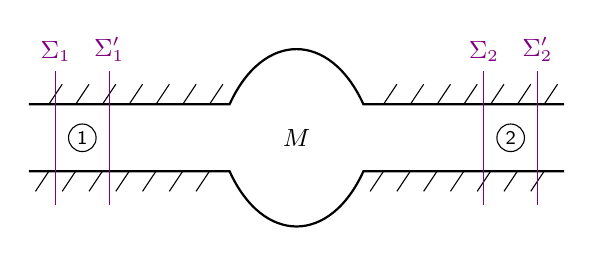
\begin{tikzpicture}[scale=.85]
\draw[thick](0,.5)--(3,.5)..controls(3.5,1.6)and(4.5,1.6)..(5,.5)--(8,.5);\draw[thick](0,-.5)--(3,-.5)..controls(3.5,-1.6)and(4.5,-1.6)..(5,-.5)--(8,-.5);\node at(4,0){$M$};
\foreach\x in{.3,.7,1.1,1.5,1.9,2.3,2.7,5.3,5.7,6.1,6.5,6.9,7.3,7.7}{\draw(\x,.5)--++(.2,.3)(\x,-.5)--++(-.2,-.3);}
\foreach\x/\lab in{.4/\Sigma_1,1.2/\Sigma'_1,6.8/\Sigma_2,7.6/\Sigma'_2}{\draw[violet](\x,-1)--(\x,1)node[above]{$\lab$};}\node at(.8,0){\zone{1}};\node at(7.2,0){\zone{2}};
\end{tikzpicture}\end{center}
\par\textbf{Hypothèses :}
\begin{itemize}
\item L'écoulement est stationnaire, donc $D_m$ est constant à travers toute section de la canalisation.
\item Les parois sont calorifugées.
\item Le fluide reçoit de la machine le travail $W_m$ et le transfert thermique $Q_m$.
\end{itemize}
\begin{cadre}[etoiles={\etoiles{5}}]
\textbf{Rappel : trois formulations du premier principe}
\begin{align*}
\Delta H+\Delta E_{m,\mathrm{macroscopique}}&=W_m+Q_m,\\
\Delta h+\Delta e_{m,\mathrm{macroscopique}}&=w_m+q_m,\\
D_m\bigl(\Delta h+\Delta e_{m,\mathrm{macroscopique}}\bigr)&=\mathcal P_u+\mathcal P_{\mathrm{th}}.
\end{align*}
\end{cadre}
\etape{1) Système fermé et bilan des forces}
Le système fermé $\Sigma$ est constitué du fluide :
\begin{itemize}\item compris entre $\Sigma_1$ et $\Sigma_2$ à $t$ ;\item compris entre $\Sigma'_1$ et $\Sigma'_2$ à $t'$.\end{itemize}
\par Le système ouvert $\sys$, fixe et indéformable, est compris entre $\Sigma'_1$ et $\Sigma_2$.
\par\par\par\medskip\noindent\begin{minipage}{\linewidth}
\textbf{Forces extérieures :}
\begin{itemize}
\item Le poids, conservatif.
\item Les forces de pression, qui fournissent les travaux d'admission et de refoulement.
\item Les forces de viscosité, dont le travail est nul car le fluide adhère aux parois.
\end{itemize}
\end{minipage}\par
\par\par\par\medskip\noindent\begin{minipage}{\linewidth}
\textbf{Forces intérieures :}
\begin{itemize}\item Les effets intérieurs sont pris en compte dans l'énergie interne.\end{itemize}
\end{minipage}\par
\etape{2) Bilan énergétique}
\[
\underset{t\to t'}{\Delta}U_\Sigma
=\underbrace{\underset{t\to t'}{\Delta}U_{\sys}}_{0}+U_2-U_1
+\underbrace{\underset{t\to t'}{\Delta}E_{m,\mathrm{macro}\,\sys}}_{0}
+E_{m,\mathrm{macro}\,2}-E_{m,\mathrm{macro}\,1}.
\]
Les variations indiquées sont prises entre $t$ et $t'$. Le travail extérieur vaut
\[W_{\mathrm{ext}}=P_1V_1-P_2V_2.\]
\etape{3) Premier principe}
\[\Delta U_\Sigma+\Delta E_{m,\mathrm{macro}\,\Sigma}=W_{\mathrm{ext}}+W_m+Q_m,\]
\[U_2-U_1+E_{m,\mathrm{macro}\,2}-E_{m,\mathrm{macro}\,1}+P_2V_2-P_1V_1=W_m+Q_m.\]
\begin{cadre}
\[\underset{t\to t''}{\Delta}H+\underset{t\to t''}{\Delta}E_{m,\mathrm{macro}}=W_m+Q_m.\]
On introduit un nouveau système fermé $\Sigma'$ : il s'agit du fluide situé dans la zone \zone{1} à l'instant $t$. On note $t''$ l'instant auquel ce même fluide occupe la zone \zone{2}. Sa masse est $D_m(t'-t)$. \\
\par Le membre de gauche correspond à la variation pour $\Sigma'$ entre $t$ et $t''$ ; le membre de droite aux échanges reçus par $\Sigma$ entre $t$ et $t'$.
\end{cadre}
Dans le cas $t'=t+\dd t$, $\Sigma'$ a pour masse $D_m\dd t$. Ainsi,
\[D_m\dd t\bigl[h_2-h_1+e_{m,\mathrm{macro}\,2}-e_{m,\mathrm{macro}\,1}\bigr]=\delta W_m+\delta Q_m.\]
\begin{cadre}\[D_m\bigl[\Delta h+\Delta e_{m,\mathrm{macro}}\bigr]=\mathcal P_u+\mathcal P_{\mathrm{th}}.\]La variation concerne $\Sigma'$ entre $t$ et $t''$ ; les puissances sont reçues par $\Sigma$.\end{cadre}
\[\Delta h+\Delta e_{m,\mathrm{macro}}=\frac{\mathcal P_u}{D_m}+\frac{\mathcal P_{\mathrm{th}}}{D_m}.\]
\begin{cadre}\[\Delta h+\Delta e_{m,\mathrm{macro}}=w_m+q_m.\]$w_m$ et $q_m$ sont le travail et la chaleur reçus par $\Sigma'$ par unité de masse de fluide qui s'écoule.\end{cadre}
\Needspace{65mm}
\subsection{Puissance d'une pompe}
% Sources 40-43
\begin{exemple}[breakable]
\begin{center}\pump{0}\end{center}
\par\textbf{Hypothèses :}
\begin{itemize}
\item Le fluide est parfait et incompressible, de masse volumique $\mu$.
\item Le régime est stationnaire.
\end{itemize}
Le rendement est
\[\eta=\frac{\text{puissance fournie par la pompe au fluide}}{\text{puissance mécanique fournie à la pompe}}.\]
\par\noindent\begin{minipage}{\linewidth}
\etape{1) Système et bilan des forces}
\begin{center}\pump{1}\end{center}
\end{minipage}\par
$\sys$ est un système ouvert fixe et indéformable.
\begin{itemize}\item $\Sigma(t)$ comprend le fluide dans $\sys$ à $t$ et le fluide entrant entre $t$ et $t+\dd t$.
\item $\Sigma(t+\dd t)$ comprend le fluide dans $\sys$ à $t+\dd t$ et le fluide sortant pendant cet intervalle.\end{itemize}
L'écoulement est stationnaire : $D_m$ est constant à travers la pompe et $\mu D_V=D_m$.
\par\par\medskip\noindent\begin{minipage}{\linewidth}
\textbf{Forces extérieures :}
\begin{itemize}\item Le poids est conservatif.
\item Les pressions amont et aval, $P_1$ et $P_2$, fournissent un travail.
\item La réaction de la canalisation sur le fluide ne travaille pas.
\item La machine fournit au fluide le travail $W_m$.\end{itemize}
\end{minipage}\par
\par\par\par\medskip\noindent\begin{minipage}{\linewidth}
\textbf{Forces intérieures :}
\begin{itemize}
\item Les forces de pression : leur travail est nul car l'écoulement est incompressible.
\end{itemize}
\end{minipage}
\\
\par \textbf{Remarque :} généralement, la canalisation ne travaille pas : soit l'écoulement est parfait et il n'y a pas de viscosité, soit le fluide adhère aux parois et il n'y a pas de mouvement relatif.
\etape{2) Bilan énergétique}
\[E_{c\Sigma}(t)=E_{c\sys}(t)+D_m\dd t\,\frac12v_1^2,\]
\[E_{c\Sigma}(t+\dd t)=E_{c\sys}(t+\dd t)+D_m\dd t\,\frac12v_2^2,\]
\[\dd E_{c\Sigma}=0+\frac12D_m\dd t(v_2^2-v_1^2),\qquad\dd E_{p\Sigma}=0+D_m\dd t(gh-0).\]
\[\dd E_{m\Sigma}=\dd E_{c\Sigma}+\dd E_{p\Sigma}=D_m\dd t\left[\frac12v_2^2-\frac12v_1^2+gh\right].\]
\etape{3) Théorème de l'énergie mécanique}
\[\dd E_{m\Sigma}=\delta W_{\mathrm{int}}+\delta W_{\mathrm{ext}},\]
\[D_m\dd t\left[\frac12v_2^2-\frac12v_1^2+gh\right]=P_1S_1v_1\dd t-P_2S_2v_2\dd t+\Pm\dd t+0.\]
Avec $D_V=S_1v_1=S_2v_2$ et $D_m=\mu D_V$,
\begin{cadre}\[\Pm=\frac{\mu D_V}{2}\left[\frac{D_V^2}{S_2^2}-\frac{D_V^2}{S_1^2}+2gh\right]+P_2D_V-P_1D_V.\]\end{cadre}
\[\mathcal P_{\mathrm{moteur}}=\frac{\Pm}{\eta}=\frac{\mu D_V}{2\eta}\left[\frac{D_V^2}{S_2^2}-\frac{D_V^2}{S_1^2}+2gh\right]+\frac{P_2D_V}{\eta}-\frac{P_1D_V}{\eta}.\]
\par\medskip\noindent\textbf{Application numérique :} $21\,\mathrm{kW}$, ordre de grandeur typique pour ce type de machine.
\end{exemple}
\section{Onde de choc}
% Sources 43-46
\titr{Idées}
\begin{itemize}\item Effectuer plusieurs bilans dans le même exercice.
\item Changer de référentiel pour obtenir un écoulement stationnaire.
\item Étudier un écoulement compressible.\end{itemize}
\begin{center}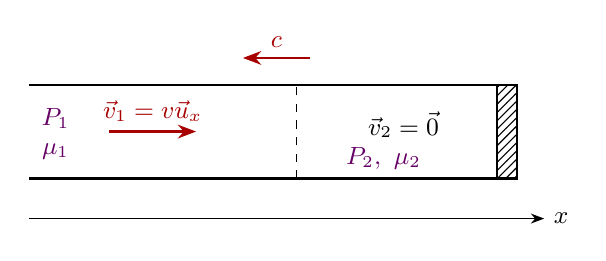
\begin{tikzpicture}[scale=.85]
\draw[thick](0,-.7)--(7,-.7)(0,.7)--(7,.7);\fill[pattern=north east lines](7,-.7)rectangle(7.3,.7);\draw[thick](7,-.7)rectangle(7.3,.7);\draw[dashed](4,-.7)--(4,.7);\draw[force](4.2,1.1)--(3.2,1.1)node[midway,above]{$c$};\draw[force](1.2,0)--(2.5,0)node[midway,above]{$\vec v_1=v\ux$};\node at(5.6,.1){$\vec v_2=\vec0$};\node[pression]at(.4,.2){$P_1$};\node[pression]at(.4,-.3){$\mu_1$};\node[pression]at(5.3,-.4){$P_2,\ \mu_2$};\draw[->](0,-1.3)--(7.7,-1.3)node[right]{$x$};
\end{tikzpicture}\end{center}
La fermeture du robinet est modélisée par une discontinuité de vitesse : une onde de choc se propage en arrière. On a $P_2>P_1$ et $\mu_2>\mu_1$.
Les inconnues sont $c$, $P_2$ et $\mu_2$. Un seul bilan ne suffit pas : il faut trois équations, issues d'un bilan de masse, d'un bilan de quantité de mouvement et d'un bilan thermodynamique.
\textbf{Remarque :} le bilan d'énergie n'est pas adapté, car l'écoulement est compressible et l'on ne connaît pas $\Piint$.
\titr{Bilan thermodynamique}
\par\textbf{Hypothèses :}
\begin{itemize}
\item L'écoulement est parfait : il n'y a pas d'échange de chaleur ni de diffusion.
\item Toutes les particules fluides ont une évolution isentropique : $S=\cste$.
\end{itemize}
$\chi_S$ est le coefficient de compressibilité isentropique.
\begin{cadre}\[\chi_S=\frac1\mu\left.\pd\mu P\right|_S.\]
Pour l'eau, $\chi_S=5\times10^{-10}\,\mathrm{Pa^{-1}}$.\end{cadre}
Rappel : $\displaystyle\chi_T=\frac1\mu\left.\pd\rho P\right|_T$.
\begin{cadre}\[\chi_S=\frac1{\mu_1}\frac{\mu_2-\mu_1}{P_2-P_1}.\tag{1}\]\end{cadre}
\begin{center}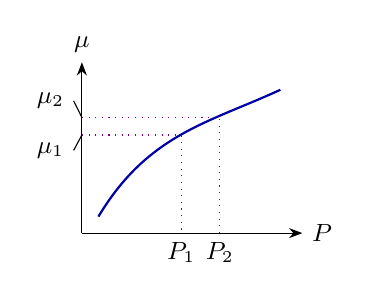
\begin{tikzpicture}[scale=.7]
\draw[->](0,0)--(4,0)node[right]{$P$};\draw[->](0,0)--(0,3.1)node[above]{$\mu$};\draw[blue!65!black,thick](.3,.3)..controls(1.2,1.8)and(2.3,2)..(3.6,2.6);\draw[violet,dotted](0,1.78)--(1.8,1.78)--(1.8,0);\draw[violet,dotted](0,2.1)--(2.5,2.1)--(2.5,0);\node[left]at(-.15,1.5){$\mu_1$};\draw[thin](-.15,1.5)--(0,1.78);\node[left]at(-.15,2.4){$\mu_2$};\draw[thin](-.15,2.4)--(0,2.1);\node[below]at(1.8,0){$P_1$};\node[below]at(2.5,0){$P_2$};
\end{tikzpicture}\end{center}
\titr{Analyse avec la mécanique des fluides}
Il faut un écoulement stationnaire : on change donc de référentiel.
On se place dans $\R'$, en translation rectiligne uniforme par rapport au référentiel galiléen du laboratoire $\R_{\mathrm{labo}}$, à la vitesse $-c\ux$. $\R'$ est galiléen.
\begin{center}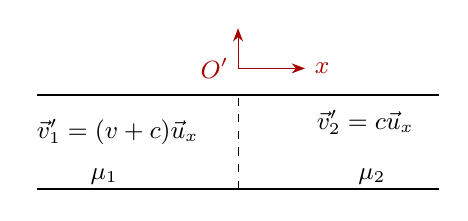
\begin{tikzpicture}[scale=.85]
\draw[thick](0,-.7)--(6,-.7)(0,.7)--(6,.7);\draw[dashed](3,-.7)--(3,.7);\draw[->,red!65!black](3,1.1)--(4,1.1)node[right]{$x$};\draw[->,red!65!black](3,1.1)--(3,1.7);\node[red!65!black,left]at(3,1.1){$O'$};\node at(1.2,.15){$\vec v'_1=(v+c)\ux$};\node at(4.9,.3){$\vec v'_2=c\ux$};\node[below]at(1,-.25){$\mu_1$};\node[below]at(5,-.25){$\mu_2$};
\end{tikzpicture}\end{center}
La composition des vitesses donne
\[v\ux=\vec v'_1-c\ux,\qquad\vec0=\vec v'_2-c\ux.\]
\titr{Bilan de masse}
Cf. partie I. Dans l'écoulement stationnaire, $D'_m=\cste$.
\begin{cadre}\[D'_m=\mu_1S(v+c)=\mu_2Sc.\tag{2}\]\end{cadre}
\titr{Bilan de quantité de mouvement}
% Sources 47-50
\par\noindent\begin{minipage}{\linewidth}
\etape{1) Système et forces extérieures}
\begin{center}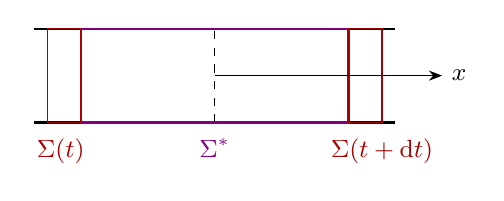
\begin{tikzpicture}[scale=.85]
\draw[thick](-.7,-.7)--(4.7,-.7)(-.7,.7)--(4.7,.7);\draw[violet,thick](0,-.7)rectangle(4,.7);\draw[dashed](2,-.7)--(2,.7);\draw[red!65!black](-.5,-.7)rectangle(0,.7);\draw[red!65!black](4,-.7)rectangle(4.5,.7);\draw[->](2,0)--(5.4,0)node[right]{$x$};\node[violet,below]at(2,-.8){$\sys$};\node[red!65!black,below]at(-.3,-.8){$\Sigma(t)$};\node[red!65!black,below]at(4.5,-.8){$\Sigma(t+\dd t)$};
\end{tikzpicture}\end{center}
\end{minipage}\par
$\sys$ est ouvert, fixe et indéformable ; $\Sigma$ est fermé.
\begin{itemize}\item À $t$, $\Sigma$ comprend le fluide contenu dans $\sys$ à $t$ et le fluide entrant entre $t$ et $t+\dd t$.
\item À $t+\dd t$, il comprend le fluide contenu dans $\sys$ à $t+\dd t$ et le fluide sortant pendant cet intervalle.\end{itemize}
\par\par\par\medskip\noindent\begin{minipage}{\linewidth}
\textbf{Forces extérieures :}
\begin{itemize}
\item Le poids, négligé.
\item Les forces de pression en amont et en aval.
\item Les forces de la canalisation sur le fluide, perpendiculaires à $\ux$.
\end{itemize}
\end{minipage}\par
\etape{2) Variation de quantité de mouvement}
\[\vec p_\Sigma(t)=\vec p_{\sys}(t)+D'_m\dd t(v+c)\ux,\]
\[\vec p_\Sigma(t+\dd t)=\vec p_{\sys}(t+\dd t)+D'_m\dd t\,c\ux,\]
\[\dd\vec p_\Sigma=\vec0+D'_m\dd t[-v]\ux.\]
\etape{3) Théorème de la quantité de mouvement projeté sur $Ox$}
\[-D'_m\dd t\,v\ux=(P_1S-P_2S)\ux\,\dd t.\]
\begin{cadre}\[D'_m v=(P_2-P_1)S.\tag{3}\]\end{cadre}
On dispose de trois équations. Leur résolution donne
\[c(c+v)=\frac1{\mu_1\chi_S}.\]
Avec l'hypothèse $c\gg v$,
\begin{cadre}\[c^2=\frac1{\mu_1\chi_S},\qquad P_2=P_1+\mu_1v(c+v).\]\end{cadre}
On obtient $\mu_2$ avec la définition de $\chi_S$, équation (1).
\titr{Application numérique}
\[v=1{,}0\,\mathrm{m\,s^{-1}},\qquad P_1=1{,}0\,\mathrm{bar},\qquad\mu_1=1{,}0\times10^3\,\mathrm{kg\,m^{-3}}.\]
On obtient $c=1{,}4\times10^3\,\mathrm{m\,s^{-1}}\gg v$ et $P_2=15\,\mathrm{bar}$.
L'onde de choc a la même vitesse que le son dans l'eau.
\textbf{Remarque :}
\[\frac1{\mu_1}\frac{\mu_2-\mu_1}{\Delta P}=\chi_S,\qquad\frac{\Delta\mu}{\mu}=\chi_S\Delta P\simeq7\times10^{-4}.\]
La variation de $\mu$ est très faible. Or l'onde de choc a pour origine la compressibilité de l'eau : il est donc impossible de considérer un écoulement incompressible.
\par\textbf{Améliorations possibles du modèle :} considérer une vitesse continue et tenir compte de la viscosité.
\par\textbf{Remarque :} $P_2=15\,\mathrm{bar}$ ; dans les robinets réels, il y a une vanne pour alléger la pression.
\end{document}